\chapter{TEXT CLASSIFICATION} \label{chapt1}
\section{Statement of the classification problem} \label{sect1_2}


A classification problem is a problem of identifying to which category a new observation belongs to. An example can be a situation when you receive a new email and the algorithm automatically decides whether it belongs to social network, promotions or business letters.


\newcommand{\docsetlabeled}{\mathbb{D}}

In text classification, we are given a description  $d \in \mathbb{X}$ of a document, where $\mathbb{X}$ is the document space ; and a fixed set of classes  $\mathbb{C} = \{ c_1,c_2,\ldots,c_J \}$. Classes are also called categories or labels . Typically, the document space  $\mathbb{X}$ is some type of high-dimensional space, and the classes are defined by people for the needs of an application, as in the examples China and documents that talk about multicore computer chips above. We are given a training set  $\docsetlabeled$ of labeled documents  $d $, where  $d \in \mathbb{X} \times \mathbb{C}$. For example: 

\begin{equation}
\label{eq:equation3}
\langle\mbox{d, c}\rangle=\langle\mbox{Beijing joins the World Trade Organization}, \emph{China}\rangle
\end{equation}
\begin{doublespacing}
\end{doublespacing}

for the one-sentence document, Beijing joins the World Trade Organization and the class (or label) China.
Using a learning method or learning algorithm , we then wish to learn a classifier or classification function  $\gamma $ that maps documents to classes:

\begin{equation}
	\label{eq:equation4}
	\gamma: \mathbb{X} \rightarrow \mathbb{C}
\end{equation}
\begin{doublespacing}
\end{doublespacing}

This type of learning is called supervised learning because a supervisor (the human who defines the classes and labels training documents) serves as a teacher directing the learning process. We denote the supervised learning method by $\Gamma$ and write  $\Gamma(\docsetlabeled) = \gamma$. The learning method $\Gamma$ takes the training set  $\docsetlabeled$ as input and returns the learned classification function $\gamma $.

The classes in text classification often have some interesting structure such as the hierarchy in Figure ~\ref{img:hierarchy}. There are two instances in each of region categories, industry categories, and subject area categories. A hierarchy can be an important aid in solving a classification problem. Our goal in text classification is high accuracy of test data or new data - for example, the newswire articles that we will encounter tomorrow morning in the multicore chip example. It is easy to achieve high accuracy on the training set (e.g., we can simply memorize the labels). But high accuracy on the training set in general does not mean that the classifier will work well on new data in the application. When we use the training set to learn a classifier for test data, we make an assumption that training data and test data are similar or from the same distribution.\cite[p.256-257]{manning}

\begin{figure}[ht] 
	\center
	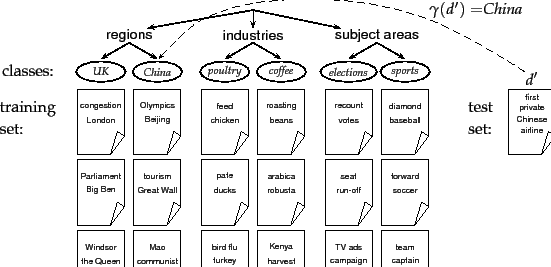
\includegraphics [scale=0.6] {hierarchy}
	\caption{Classes, training set, and test set in text classification.} 
	\label{img:hierarchy}  
\end{figure}


\section{Short review of existing mathematical model which can be used to solve the classification problem} \label{sect1_3}

\begin{figure}[ht] 
	\center
	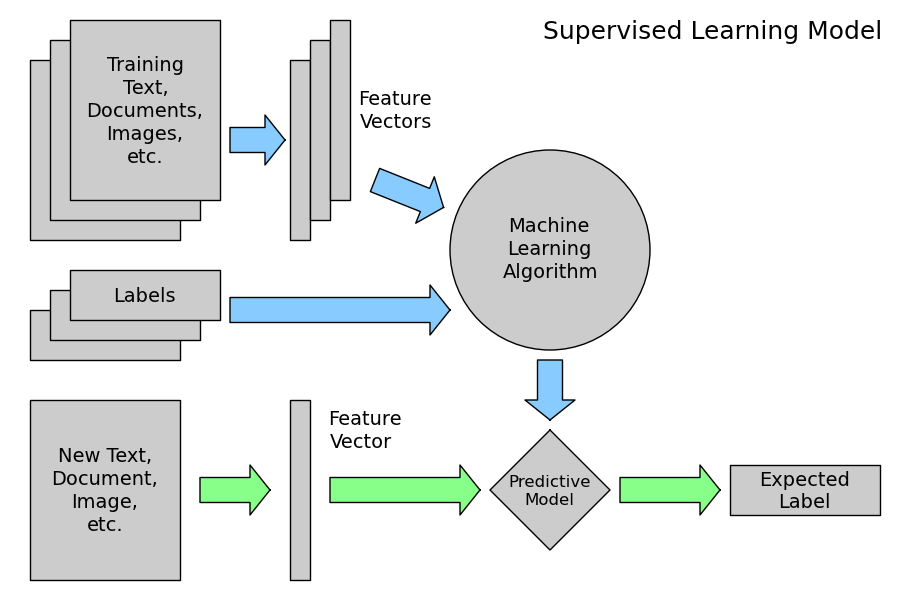
\includegraphics [scale=0.6] {work_flow}
	\caption{Supervised learning workflow.} 
	\label{img:supervised_learning_work_flow}  
\end{figure}

Supervised learning is the machine learning task of inferring a function from labelled training data. The training data consist of a set of training examples. Between inputs and reference outputs there may be some dependence, but it is unknown. On the basis of these data, it is necessary to restore the dependence. In order to measure the accuracy, a quality function can be introduced.\cite[p.7]{foundationsml} The diagram of the supervised learning process is presented in Figure ~\ref{img:supervised_learning_work_flow} 
\\

\noindent Here are some of the most important supervised learning algorithms:
\begin{enumerate}
	\item Naive Bayes .\cite{NB1}.\cite{NB2}
	%\item k-Nearest Neighbors
	\item Logistic Regression .\cite{LR}
	\item Support Vector Machines (SVMs) .\cite{svm}
	\item Decision Trees and Random Forests .\cite{manning}
	\item Neural networks .\cite{manning}
\end{enumerate}


\section{Model evaluation and validation} \label{sect1_4}
Machine learning pipeline is not finished with a model evaluation. We want to estimate correctly future data by using special techniques and metrics that are suitable for a particular task.

Now let us find out what validation is for?
\begin{enumerate}
	\item Validation helps to evaluate model performance, its quality, its ability to generalise.
	\item Validation can be used to select the best model to perform on unseen data.
	\item Overfitting of the model leads to the inconsistent and poor performance of the model on future data.
\end{enumerate}

To better understand each point we need to examine it more deeply.

\subsection{Model Evaluation Applications}
A very important property of learning models is Generalization performance. In general, we want to estimate the predictive performance of our model on future data.  Therefore, it is necessary to use special techniques and metrics that are suitable for a particular task to track the performance of our models. 

When we have a set of candidate models, model selection helps us to increase the predictive performance by tweaking the learning algorithm and selecting the best performing model from a given hypothesis space.
 
Before machine learning engineers find the best model, they make a bunch of experiments. Running a learning algorithm over a training dataset with different hyperparameter settings and various features will result in different models. The final goal is to select the best one from the set, ranking their performances against each other.

Algorithm selection - in most cases we deal with many algorithms to find the best one under the given circumstances. Therefore, we naturally need to compare different algorithms to each other, often regarding predictive and computational performance.
Nevertheless, these three sub-tasks have some similarities. When we want to estimate the performance of a model, they all require different approaches.


\subsection{Model Evaluation Techniques}
Holdout method (simple train/test split)
The holdout method is the most straightforward model evaluation technique. We take our labelled dataset and split it randomly into two parts: a training set and a test set.Then, we fit a model to the training data and predict the labels of the test set. And the fraction of correct predictions reflects our estimate of the prediction.

\begin{figure}[h!] 
	\center
	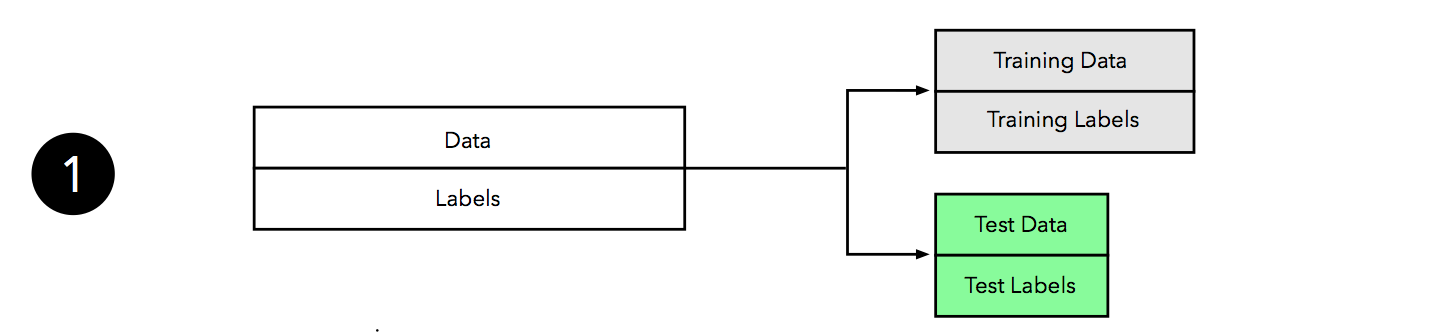
\includegraphics [scale=1] {eval1}
	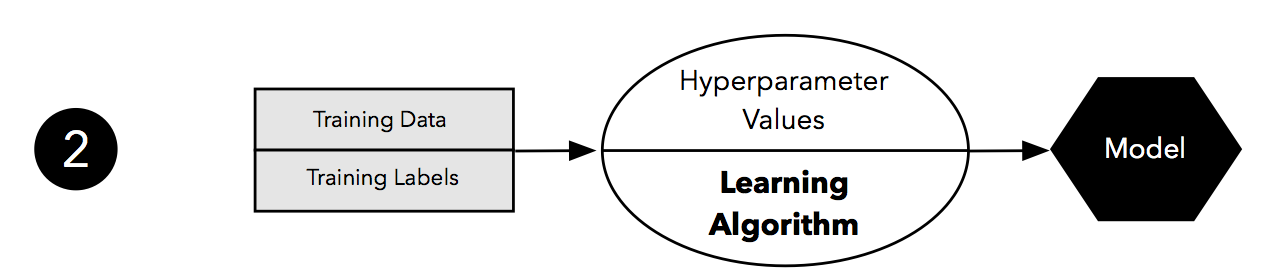
\includegraphics [scale=1] {eval2}
	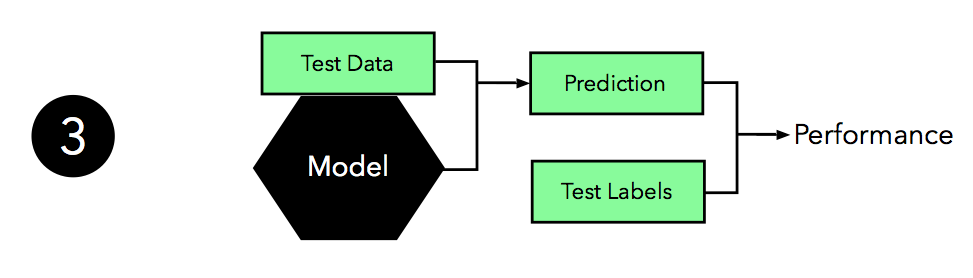
\includegraphics [scale=1] {eval3}
	\caption{Holdout method} 
	\label{img:eval3}  
\end{figure}

We don’t want to train and evaluate our model on the same training dataset, because it will lead to overfitting - the model will simply memorise the training data, and it will generalise wrong to unseen data. \cite{model_evaluation}


\section{Classification metrics}

Classification problems are probably the most common type of ML problem, and therefore many metrics can be used to evaluate predictions of these problems. The most frequently used metrics for classification problems are:

\begin{enumerate}
	\item Accuracy \ref{accuracy} \\
	Accuracy simply measures what percent of your predictions is correct. It is the ratio between the number of correct predictions and the total number of predictions.
	
	\begin{equation}
	\label{accuracy}
	accuracy = {\frac{correct}{predictions}}
	\end{equation}
\begin{doublespacing}
\end{doublespacing}
	
	Accuracy measures merely what percent of forecasts are correct. Accuracy is also the most misused metric. It is actually only suitable when there is an *equal number of observations in each class* (which is rarely the case) and that all *predictions and prediction errors are equally important, which is often not the case.
	
	\item Confusion Matrix 1.4 \\
	The confusion matrix is a handy presentation of the accuracy of a model with 2 or more classes. The table presents predictions on the x-axis and accuracy outcomes on the y-axis. The cells of the table are the number of predictions made by a machine learning algorithm.
	
	\newcommand\MyBox[2]{
		\fbox{\lower0.75cm
			\vbox to 1.7cm{\vfil
				\hbox to 2.2cm{\hfil\parbox{1.4cm}{#1\\#2}\hfil}
				\vfil}%
		}%
	}
	
	\noindent
	\begin{figure}[ht] 
		\center
		\label{img:CM} 
		\renewcommand\arraystretch{1.5}
		\setlength\tabcolsep{0pt}
		\begin{tabular}
			{c >{\bfseries}r @{\hspace{0.8em}}c @{\hspace{0.4em}}c @{\hspace{0.7em}}l}
			\multirow{10}{*}{\parbox{1.1cm}{\bfseries\raggedleft actual\\ value}} & 
			& \multicolumn{2}{c}{\bfseries Prediction outcome} & \\
			& & \bfseries p & \bfseries n & \bfseries total \\
			& p$'$ & \MyBox{True}{Positive} & \MyBox{False}{Negative} & P$'$ \\[2.4em]
			& n$'$ & \MyBox{False}{Positive} & \MyBox{True}{Negative} & N$'$ \\
			& total & P & N &
		\end{tabular}	
		\caption{Confusion matrix} 
		 
	\end{figure}
	
	Confusion matrix allows one to compute various classification metrics.
	
	\item Precision \ref{precision} and Recall \ref{recall}\\
	Precision and recall are two metrics. But they are often used together.
	Precision answers the question: What percent of positive predictions was correct?
	
	\begin{equation}
	\label{precision}
	precision = {\frac{\#\ true\ positive}{\#\ true\ positive + \#\ false\ positive}}
	\end{equation}
\begin{doublespacing}
\end{doublespacing}
	
	Recall answers the question: What percent of the positive cases did you catch?
	
	\begin{equation}
	\label{recall}
	recall = {\frac{\#\ true\ positive}{\#\ true\ positive + \#\ false\ negative}}
	\end{equation}
\begin{doublespacing}
\end{doublespacing}
	
	\item F1-score \ref{f1}\\
	The F1-score (sometimes known as the balanced F-beta score) is a single metric that combines both precision and recall via their harmonic mean:
	
	\begin{equation}
	\label{f1}
	F_1 = 2 {\frac{precision * recall}{precision + recall}}
	\end{equation}
\begin{doublespacing}
\end{doublespacing}
	
	Unlike the arithmetic mean, the harmonic mean tends toward the smaller of the two elements. Hence the F1 score will be small if either precision or recall is small.
\end{enumerate}

\section{Summary of the section}

In the first section the relevance of the problem and the main concepts associated with it are considered, namely, classification, its formation, intellectual analysis. It is a review of the main methods and algorithms of classification and criteria for its management.

Since it is important to investigate not only the ways to classify texts, but also attempt to understand main features, which had the highest importance. It is important to study the theory of how to represent textual information before applying algorithms. Then, from the examined algorithms, deep neural networks will be used. 

With the criterion for further work, the top-5 accuracy and F1-score curve were selected.
